%% Do not edit unless you really know what you are doing.
\documentclass[french,english,12pt]{exam}

\printanswers

\usepackage{../../latex/macro_mealor}
\usepackage[utf8]{inputenc}
\usepackage[T1]{fontenc} % accents codés dans la fonte
%\usepackage{layout}
\usepackage{a4wide}
%\usepackage[french]{babel}
\usepackage{hyperref}

\usepackage{graphicx}
\usepackage{caption}

\usepackage{newpxtext,newpxmath}
\usepackage{siunitx}

%\setlength{\hoffset}{0pt}
%\setlength{\oddsidemargin}{-1cm}   % Marge gauche sur pages impaires
%\setlength{\evensidemargin}{-1cm}   % Marge gauche sur pages paires
%\setlength{\marginparwidth}{0cm}   % Largeur de note dans la marge
%\setlength{\textwidth}{16cm}   % Largeur de la zone de texte (17cm)
\setlength{\voffset}{0pt}   % Bon pour DOS
\setlength{\marginparsep}{0pt}   % Séparation de la marge
\setlength{\topmargin}{0cm}   % Pas de marge en haut
\setlength{\headheight}{0cm}   % Haut de page
\setlength{\headsep}{0cm}   % Entre le haut de page et le texte
%\setlength{\footskip}{1cm}   % Bas de page + séparation
%\setlength{\textheight}{25.5cm}   % Hauteur de la zone de texte (25cm)

\usepackage{indentfirst}


\newcommand{\classurl}{\url{1}}
% #1 numéro de la feuille
% #2 titre de la feuille
\newcommand{\titre}[3] {%\textit{
  \begin{center}\textbf{\textsc{MEALOR II}}\\ \textit{Mécanique de l'endommagement et approche locale de la rupture}%\let\thefootnote\relax\footnotetext{\classurl} 
  \end{center}
 
  \noindent TD n\textdegree #1 \hfill  August 2023\\[-0.3cm]
  \rule{\linewidth}{.3mm}
  \vspace*{0.5pt}
  \begin{center}
    {
      \Large \bfseries { #2}
    }\\
    \vspace*{0.5cm}
	\large #3
    \vspace*{0.5cm}
  \end{center}
}

\usepackage{xcolor}
\definecolor{Blue}{RGB}{0,68,170}
\SolutionEmphasis{\normalfont\color{Blue}}
\DeclareCaptionFont{blue}{\color{Blue}}

\newenvironment{objectifs}
    {\itshape\underline{Objectifs:}\begin{itemize}
    }
    { \itshape
    \end{itemize}
    }
    
\newcounter{Rfig}
\newenvironment{R_figure}
   {\begin{minipage}{\linewidth}\begin{center}\vspace{0.5mm}\stepcounter{Rfig}\addtocounter{figure}{-1}\renewcommand\thefigure{R-\arabic{Rfig}}
   \captionsetup{font=blue}}
   {\end{center}\vspace{0.5mm}\end{minipage}}
   
    
\newcounter{Rtab}
\newenvironment{R_table}
   {\begin{minipage}{\linewidth}\begin{center}\vspace{0.5mm}\stepcounter{Rtab}\addtocounter{table}{-1}\renewcommand\thetable{R-\arabic{Rtab}}
   \captionsetup{font=blue}
}
   {\end{center}\vspace{0.5mm}\end{minipage}}
   
      
\graphicspath{{./pic/}}

\begin{document}
\thispagestyle{empty}
\titre{1}{Modèles de rupture fragile}{Jérémy Bleyer, Anne-Françoise Gourgues-Lorenzon}
%\maketitle
\begin{objectifs}
\item Appliquer les concepts du modèle de Griffith par la méthode de la souplesse
\item \'Evaluer un critère de propagation de fissure et discuter de la stabilité de la propagation 
\item Modèle de Beremin
\end{objectifs}

\section{Théorie de Griffith: essai \textit{End-Notched Flexure} (ENF)}


L'essai ENF (End-Notched Flexure) consiste en une flexion 3 points d'une poutre entaillée à mi-hauteur par une préfissure de longueur initiale $a_0$ débouchant à une des extrémités de la poutre (Figure \ref{fig:ENF}). Cet essai est notamment utilisé pour caractériser les propriétés de délaminage d'interface des matériaux composites multicouches.

La poutre de longueur $L$, de hauteur $2h$ et de largeur $b$, est simplement appuyée à ses extrémités et chargée par un effort ponctuel vertical $F$ appliqué au centre de la poutre. On note $\Delta$ le déplacement vertical du point d'application de la force. Une expression analytique approchée de la relation force/déplacement peut-être obtenue à l'aide d'une modélisation simplifiée reposant sur la théorie des poutres d'Euler-Bernoulli \cite{allix}. Pour une fissure de taille $a$ fixée, la relation force/déplacement s'exprime comme:
\begin{equation}
\Delta = \begin{cases}
\dfrac{L^3/12 + a^3}{32EI}F & \text{si } a\leq L/2\\
\dfrac{L^3/3 - (L-a)^3}{32EI}F & \text{si } a\geq L/2
\end{cases}
\end{equation}
où $EI = Ebh^3/12$ est la raideur en flexion d'une moitié de poutre.


\begin{figure}[h]
\begin{center}
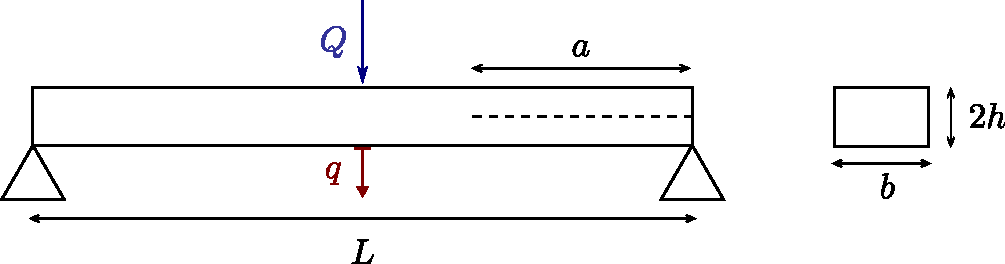
\includegraphics[width=0.8\textwidth]{ENF}
\end{center}
\caption{Essai ENF}\label{fig:ENF}
\end{figure}

\begin{questions}
\question Quel est le mode principal de sollicitation de la fissure ?
\begin{solution}
Sur appui, la fissure est sollicitée principalement par des contraintes de cisaillement, soit une fissuration en mode II.
\end{solution}
\end{questions}

\subsection{Rappels préliminaires}
\begin{questions}

\question En notant $C(a)=\Delta/F$ la souplesse de la structure à longueur $a$ de fissure fixée, donner la valeur de l'énergie potentielle de la solution suivant que l'on pilote: (a) en force, (b) en déplacement.
\begin{solution}
Par définition de la souplesse, l'énergie élastique vaut:
$$E_\text{el}=\dfrac{1}{2}C(a)F^2$$
Lorsque l'on pilote en force, on donc:
$$E_\text{pot} = E_\text{el}-W_\text{ext} = \dfrac{1}{2}C(a)F^2 - F\Delta = -\dfrac{1}{2}C(a)F^2$$
tandis que si l'on pilote en déplacement:
on a:
$$E_\text{pot} = E_\text{el} = \dfrac{1}{2}C(a)F^2 = \dfrac{1}{2}\dfrac{\Delta^2}{C(a)}$$
notons que dans ce cas, on a réexprimé l'énergie potentielle en fonction du paramètre de chargement, ici le déplacement $\Delta$.
\end{solution}
\question En déduire le taux de resitution d'énergie $\mathcal{G}$ dans les deux modes de pilotage de chargement.
\begin{solution}
De manière générale:
$$\mathcal{G} = -\dfrac{dE_\text{pot}}{dS} = -\dfrac{1}{b}\dfrac{dE_\text{pot}}{da}$$
On a alors pour un pilotage en force:
$$\mathcal{G} =  \dfrac{1}{2b}C'(a)F^2$$
et pour un pilotage en déplacement:
$$\mathcal{G} =  \dfrac{1}{2b}C'(a)\left(\dfrac{\Delta}{C(a)}\right)^2=\dfrac{1}{2b}C'(a)F(a)^2$$
\end{solution}
\question Rappeler la condition de propagation et de stabilité/instabilité de propagation de la fissure.
\begin{solution}
Il y a propagation lorsque $\mathcal{G}=\mathcal{G}_c$. La propagation sera stable si $\mathcal{G}'(a) < 0$ tandis qu'elle sera instable sinon.
\end{solution}
\end{questions}

\subsection{Application à l'essai ENF: pilotage en force}

Dans cette section, on se limite au \textbf{pilotage en force}.

\begin{questions}
\question Dans le cas $a\leq L/2$, déterminer la condition de propagation de la fissure. Discuter du caractère stable ou instable de la propagation.
\begin{solution}
On a ici:
$$C'(a) = \dfrac{3a^2}{32EI} \quad \text{soit } \mathcal{G}=\dfrac{3F^2a^2}{64bEI}$$
Ainsi, la fissure ne se propage pas tant que:
$$F \leq F_c = \sqrt{\dfrac{64bEI\mathcal{G}_c}{3a_0^2}}$$
Au delà de $F_c$, comme $\mathcal{G}'(a_0) >0$, la propagation est instable.
\end{solution}
\question Faire de même pour le cas $a \geq L/2$.
\begin{solution}
On a dans ce cas:
$$C'(a) = \dfrac{3(L-a)^2}{32EI} \quad \text{soit } \mathcal{G}=\dfrac{3F^2(L-a)^2}{64bEI}$$
Ainsi, la fissure ne se propage pas tant que:
$$F \leq F_c = \sqrt{\dfrac{64bEI\mathcal{G}_c}{3(L-a_0)^2}}$$
Au delà de $F_c$, comme 
$$\mathcal{G}'(a_0) =  -\dfrac{6F^2(L-a_0)}{64bEI}<0,$$ la propagation est stable.
\end{solution}
\end{questions}

\subsection{Application à l'essai ENF: pilotage en déplacement}

Dans cette section, on se limite au \textbf{pilotage en déplacement} et au cas $a\leq L/2$.

\begin{questions}
\question Déterminer la condition de propagation de la fissure. 
\begin{solution}
On a toujours:
$$C'(a) = \dfrac{3a^2}{32EI} \quad \text{soit } \mathcal{G}=\dfrac{48EI\Delta^2}{b}\dfrac{a^2}{(L^3/12+a^3)^2}$$
Ainsi, la fissure ne se propage pas tant que:
$$\Delta \leq \Delta_c = \sqrt{\dfrac{b\mathcal{G}_c}{48EI}}\dfrac{L^3/12+a_0^3}{a_0}$$
\end{solution}
\question Discuter du caractère stable ou instable de la propagation. On pourra pour cela s'appuyer sur le graphe de la fonction $f(x) = \dfrac{x^2}{(1/12+x^3)^2}$ représenté sur la Figure \ref{fig:graphe-fonction}.
\begin{figure}
\begin{center}
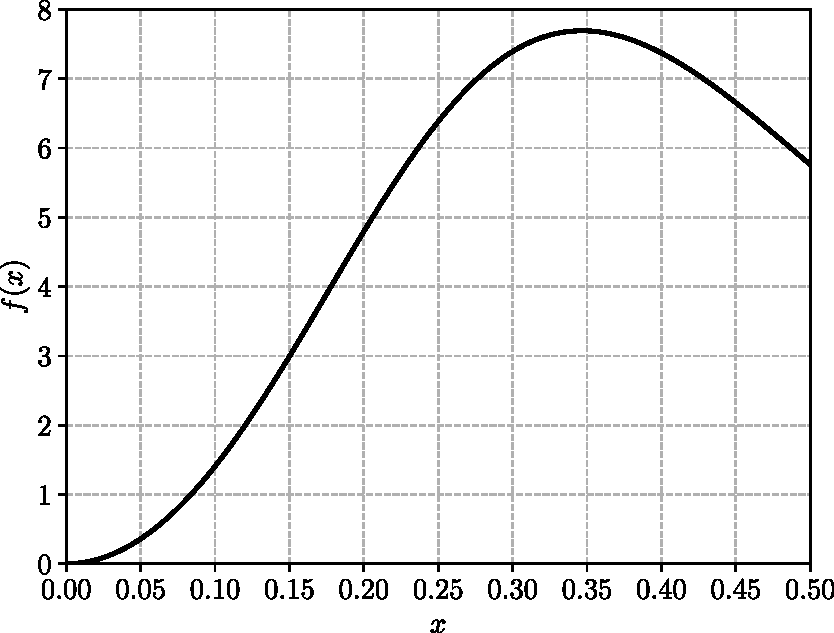
\includegraphics[width=0.65\textwidth]{function_variation}
\end{center}
\caption{Graphe de la fonction $f(x) = \dfrac{x^2}{(1/12+x^3)^2}$}\label{fig:graphe-fonction}
\end{figure}
\begin{solution}
Au delà de $\Delta_c$, la stabilité est conditionnée par le signe de $\mathcal{G}'(a_0)$ qui est lié au signe de $f'(a_0/L)$ pour la fonction $f$ indiquée par l'énoncé. Graphiquement, on trouve que cette dérivée est positive si $a_0/L < 0.35$ environ, correspondant à une propagation instable. Pour des fissures initialement plus grandes que $0.35L$ la propagation est stable.

Notons que l'étude de variation exacte de la fonction conduit à la condition $a_0 \geq \left(\frac{1}{24}\right)^{1/3}L \approx 0.347L$. Ces différentes conditions de stabilité se traduisent également dans l'évolution de la courbe force/déplacement suivant la taille de la préfissure.

\begin{R_figure}
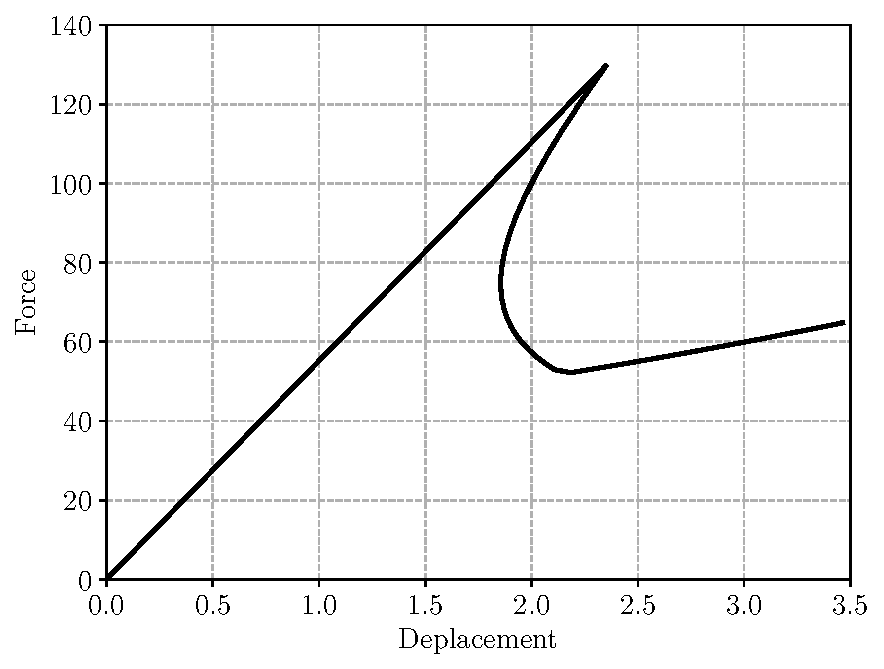
\includegraphics[width=0.49\textwidth]{ENF_force_deplacement_0.2L}
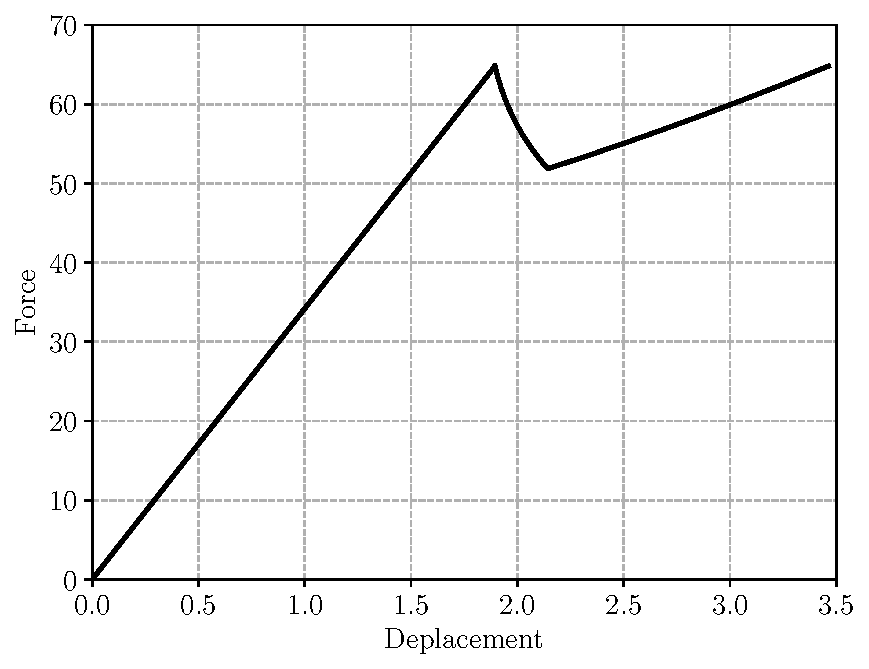
\includegraphics[width=0.49\textwidth]{ENF_force_deplacement_0.4L}\\
Force/déplacement à déplacement contrôlé pour différentes longueurs initiales de fissure. Gauche: $a_0=0.2L$ (instable); droite: $a_0=0.4L$ (stable)
\end{R_figure}

\end{solution}
\end{questions}

\begin{thebibliography}{9}
\bibitem{allix}
O. Allix, P. Ladeveze, A. Corigliano, Damage analysis of interlaminar fracture specimens, Composite Structures 31 (1995)
61–74.
\end{thebibliography}

\end{document}
